\section{Распознавание языка документов (вариант 7)}
\label{sec:langdetect}

\subsection{Постановка задачи}

В соответствии с вариантом~7 система расширена подсистемой распознавания
языка документа. Распознаются два языка "--- \textbf{французский} и
\textbf{английский}; формат входных документов "--- \textbf{HTML}.
Реализованы три метода, предусмотренные методическими указаниями:

\begin{enumerate}
	\item метод N-грамм (Кавнар "--- Тренкле, out-of-place);
	\item алфавитный метод (диакритика + слова-маркеры);
	\item нейросетевой метод (логистическая регрессия на символьных TF-IDF).
\end{enumerate}

Итоговое решение принимается \textbf{голосованием большинства} трёх методов;
дополнительно возвращается флаг \texttt{agreed} (все три метода сошлись).
Существующая клиент-серверная архитектура переиспользована: парсинг и
предобработка вынесены в отдельный языковой тракт, не затрагивающий
поисковый конвейер (чей \texttt{clean\_text} оставляет только символы
\texttt{a--z} и тем самым уничтожал бы французскую диакритику).

\subsection{Обучающая и тестовая коллекции}

Обучающие корпуса и тестовая коллекция генерируются скриптом
\texttt{backend/build\_lang\_corpus.py} детерминированно (seed~=~7, метод
дополнения "--- тасование с повторением абзацев) из автономных текстовых
заготовок (\texttt{backend/lang\_seeds.py}); интернет для генерации не
требуется. Состав коллекций приведён в таблице~\ref{tab:lang_collections}.

\begin{table}[H]
	\caption{Состав обучающей и тестовой коллекций.}
	\label{tab:lang_collections}
	\begin{tabular}{|l|l|l|}
		\hline
		Коллекция & Объём & Источник / примечание \\ \hline
		\texttt{training/en.txt} & 36,4 Кб & 10 энциклопедических абзацев (EN), seed~=~7 \\
		\texttt{training/fr.txt} & 36,4 Кб & 10 энциклопедических абзацев (FR), seed~=~7 \\
		\texttt{test\_html/} (5 EN + 5 FR) & $\approx$2,5--2,9 тыс. символов каждый ($\approx$А4) &
		Абзацы, не пересекающиеся с обучающими (held-out) \\
		\texttt{manifest.csv} & --- & Истинные метки \texttt{true\_lang} тестовых файлов \\
		\texttt{corpus\_meta.json} & --- & Метод, seed, размеры (для воспроизводимости) \\ \hline
	\end{tabular}
\end{table}

Тестовые абзацы не пересекаются с обучающими, что исключает утечку
обучающих данных в тест. Каждый тестовый документ "--- валидный HTML
(\texttt{<html><head><body>}, часть файлов содержит шумовые блоки
\texttt{<script>}/\texttt{<style>} для проверки парсера).
Методика рекомендует корпуса 20--120~Кб на язык: текущий объём (36,4~Кб)
удовлетворяет нижней границе; заготовки могут быть заменены статьями
Википедии без изменения кода.

\subsection{Архитектура подсистемы}

Языковой тракт реализован пятью модулями (каталог \texttt{backend/}):

\begin{itemize}
	\item \texttt{lang\_text.py} "--- извлечение текста из \texttt{<body>} HTML и предобработка с сохранением диакритики; нарезка на чанки; подсчёт accuracy/confusion;
	\item \texttt{lang\_ngram.py} "--- профили топ-300 и дистанция out-of-place (только стандартная библиотека);
	\item \texttt{lang\_alphabet.py} "--- диакритика, маркеры, подбор порога (только стандартная библиотека);
	\item \texttt{lang\_detect.py} "--- обучение и классификация LogReg на символьных TF-IDF (требует scikit-learn);
	\item \texttt{lang\_methods.py} "--- оркестратор: обучение всех методов, классификация с голосованием, пакетная оценка с метриками по каждому методу.
\end{itemize}

Языковые профили хранятся файлами в \texttt{backend/lang\_profiles/}
(\texttt{ngram\_en.json}, \texttt{ngram\_fr.json}, \texttt{alphabet.json},
\texttt{ml\_model.pkl}) с кэшированием в памяти и инвалидацией по mtime;
таблицы БД при этом не изменяются (векторные таблицы размерности 5000
к задаче отношения не имеют). Сервер предоставляет четыре эндпоинта:
\texttt{GET /api/lang/status}, \texttt{POST /api/lang/train},
\texttt{POST /api/lang/classify} (файл или JSON \texttt{\{text\}}),
\texttt{POST /api/lang/classify-batch}. При старте модель дообучается
автоматически, если корпуса на месте (\texttt{\_ensure\_lang\_model}),
причём сбой обучения никогда не прерывает запуск сервера.

Сценарии обучения, одиночной и пакетной классификации показаны на
рисунках~\ref{fig:lang_train_seq}--\ref{fig:lang_batch_seq}
(исходники "--- \texttt{plantuml/sequence\_lang\_*.puml}).

\begin{figure}[H]
	\centering
	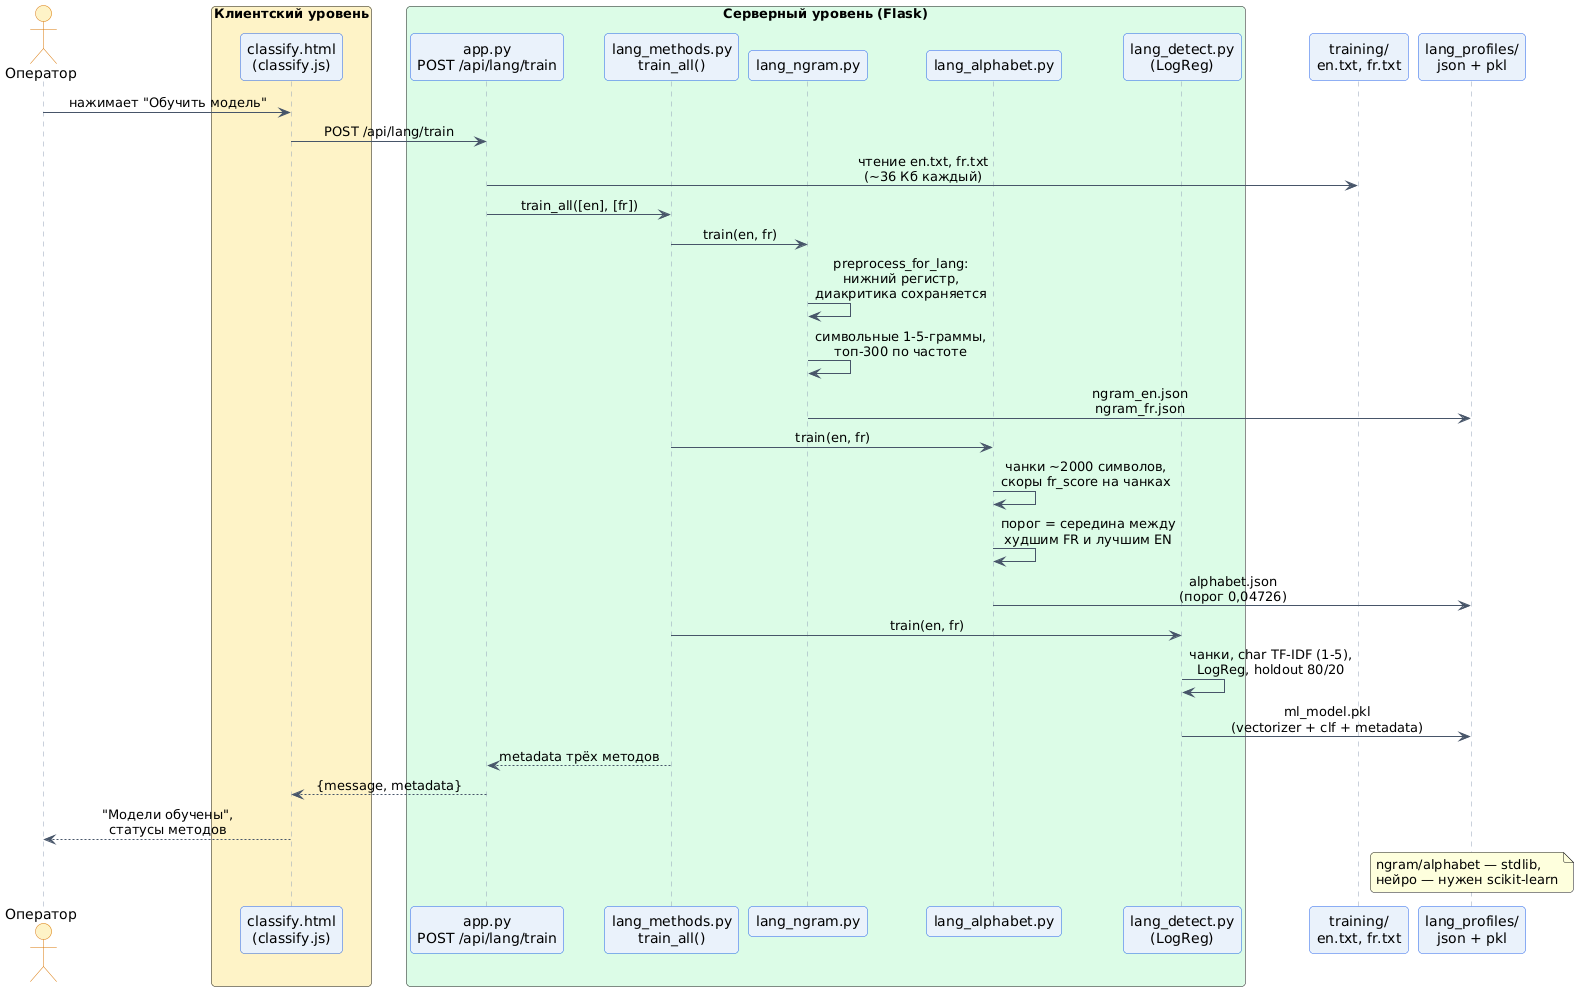
\includegraphics[width=1.0\textwidth]{png/sequence_lang_train.png}
	\caption{Диаграмма последовательности обучения трёх методов.}
	\label{fig:lang_train_seq}
\end{figure}

\begin{figure}[H]
	\centering
	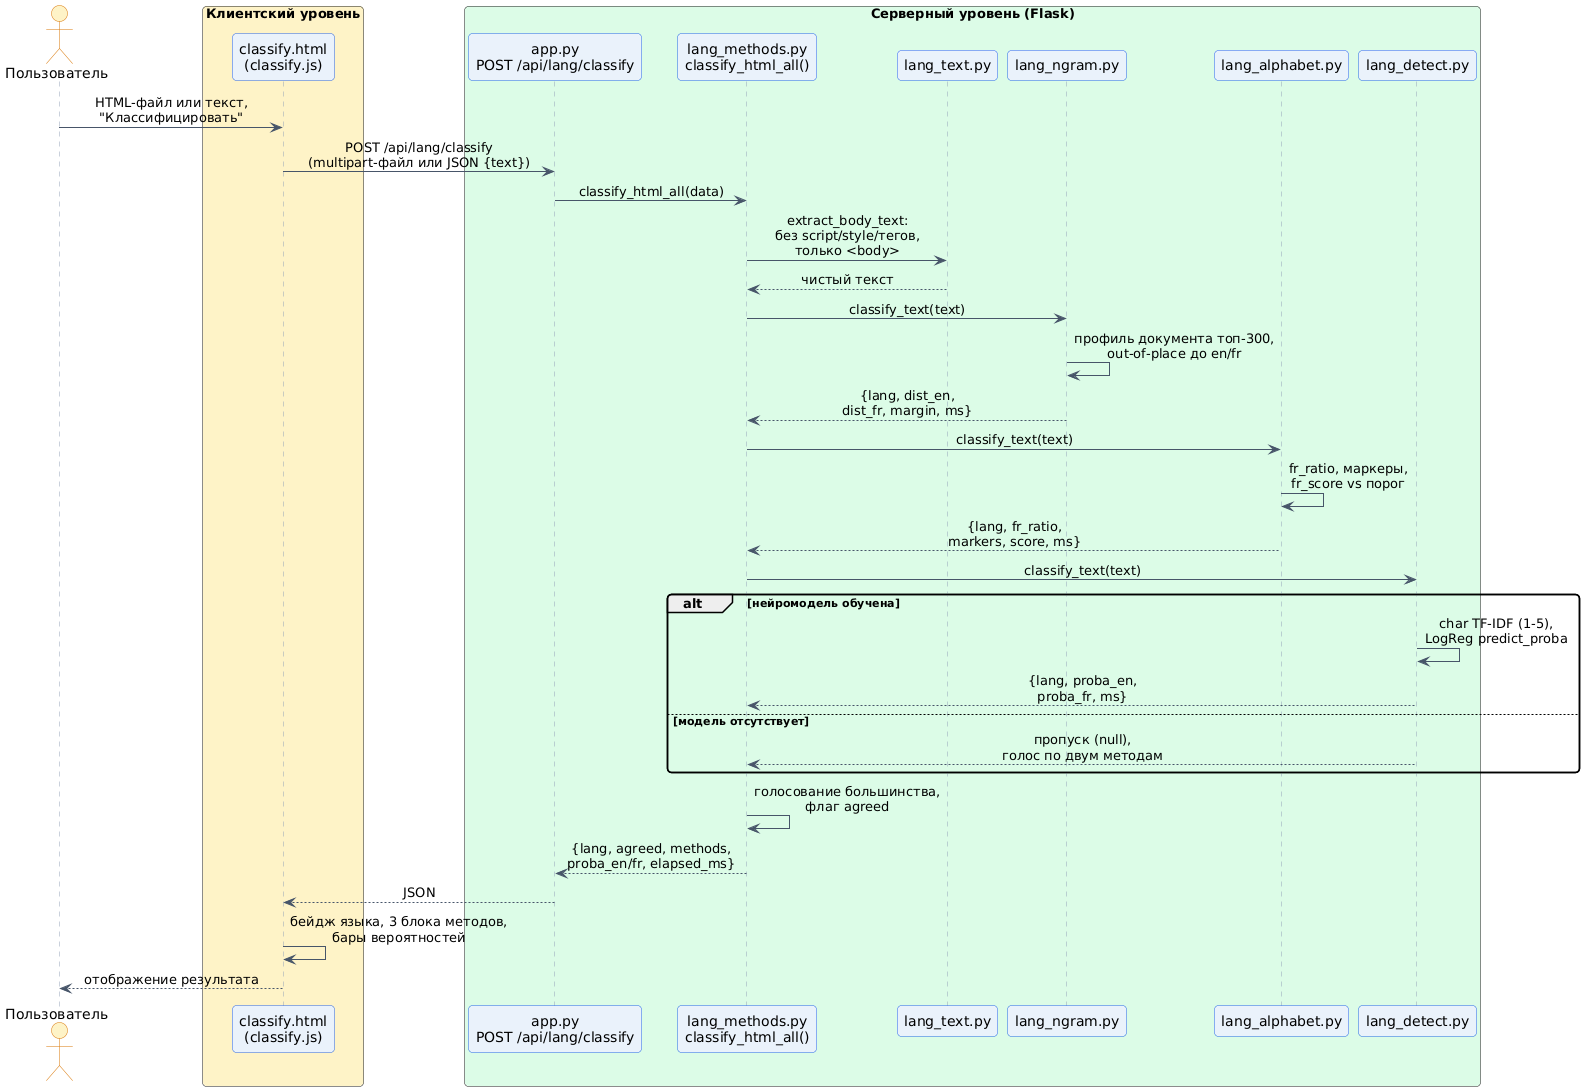
\includegraphics[width=1.0\textwidth]{png/sequence_lang_classify.png}
	\caption{Диаграмма последовательности классификации одного документа.}
	\label{fig:lang_classify_seq}
\end{figure}

\begin{figure}[H]
	\centering
	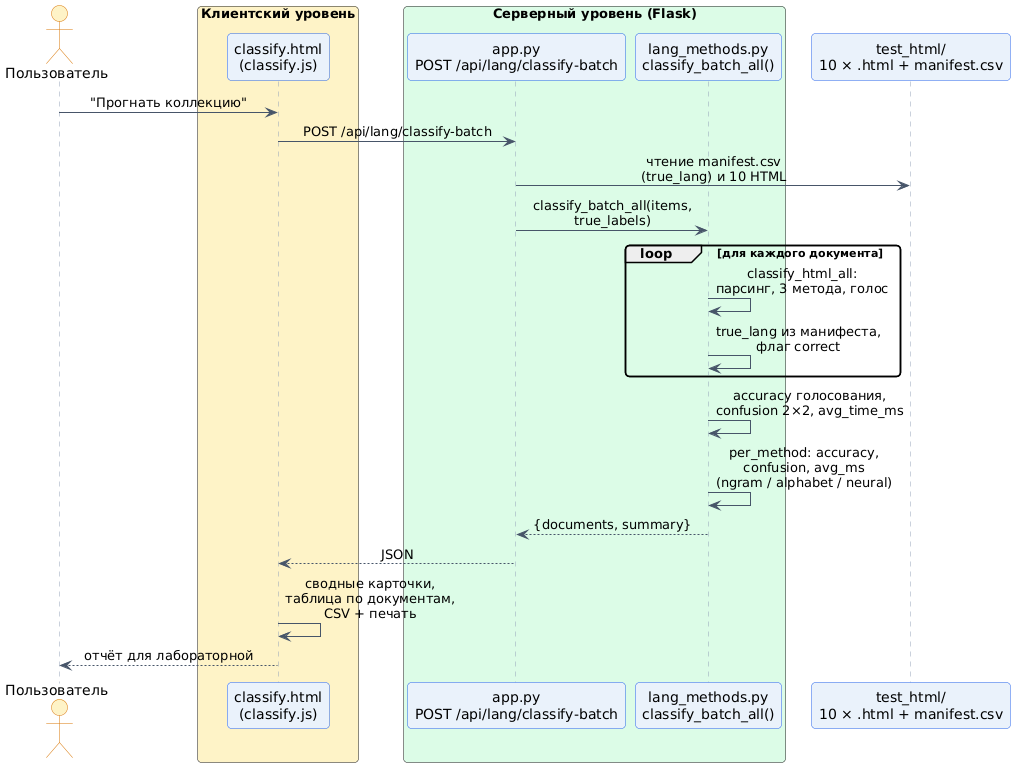
\includegraphics[width=1.0\textwidth]{png/sequence_lang_batch.png}
	\caption{Диаграмма последовательности пакетной классификации коллекции.}
	\label{fig:lang_batch_seq}
\end{figure}

Клиентская часть "--- страница \texttt{classify.html}: статус моделей,
одиночная проверка (файл или текст), прогон коллекции со сводной таблицей
(точность, confusion matrix, среднее время), выгрузка отчёта в CSV и печать.
Страница справки \texttt{help.html} "--- статическая справка с боковым
меню навигации, теория разбита по разделам.

\subsection{Интеграция с системой поиска}

Классификатор языка интегрирован в поисковый конвейер:

\begin{itemize}
	\item при загрузке документа (API \texttt{/api/upload}, \texttt{/api/upload-file})
	вызывается функция \texttt{\_classify\_lang()}, результат записывается
	в колонку \texttt{lang} таблицы \texttt{documents};
	\item при загрузке всего корпуса (\texttt{/api/init-db}) каждый документ
	классифицируется и получает метку языка;
	\item при обработке событий файлового наблюдателя язык классифицируется
	автоматически;
	\item при поиске язык запроса определяется тем же классификатором
	(\texttt{\_detect\_lang()} в \texttt{search\_engine.py}) и передаётся
	в поисковую функцию;
	\item предобработка текста определяется параметром \texttt{lang}:
	для английского --- стемминг Портера и английские стоп-слова,
	для французского --- без стемминга, с сохранением диакритики
	и французскими стоп-словами.
\end{itemize}

Таким образом, система корректно обрабатывает документы на обоих языках
и автоматически выбирает режим предобработки в зависимости от языка
документа или запроса.

\subsection{Парсинг HTML и предобработка}

Извлечение текста (\texttt{lang\_text.extract\_body\_text}):

\begin{enumerate}
	\item удаление блоков \texttt{<script>}, \texttt{<style>}, \texttt{<noscript>} вместе с содержимым;
	\item выделение содержимого \texttt{<body>} (при отсутствии "--- весь документ);
	\item удаление остальных тегов, раскрытие HTML-сущностей, нормализация пробелов.
\end{enumerate}

Предобработка (\texttt{lang\_text.preprocess\_for\_lang}): приведение
к нижнему регистру, удаление цифр и пунктуации \textbf{с сохранением}
французских букв \texttt{àâäéèêëîïôöùûüçœæÿ}. Для обучения корпус
дополнительно режется на чанки $\approx$2000 символов по границам
предложений (19 чанков EN, 18 чанков FR).

\subsection{Метод N-грамм}

Профиль языка "--- упорядоченный список топ-$K$ ($K = 300$) символьных
n-грамм ($n = 1\ldots5$, паддинг пробелами) по частоте на обучающем
корпусе. Профиль документа строится аналогично. Расстояние out-of-place:

\begin{equation}
	D(d, L) = \sum_{i} \begin{cases}
		|r_d(g_i) - r_L(g_i)|, & g_i \in L, \\
		K, & g_i \notin L,
	\end{cases}
	\label{eq:lang_oop}
\end{equation}

где $r_d$, $r_L$ "--- ранги n-граммы в профилях документа и языка;
отсутствующей n-грамме начисляется штраф $K = 300$.
Выбирается язык с минимальной дистанцией; дополнительно возвращается
разность дистанций \texttt{margin}. Блок-схема "--- на
рисунке~\ref{fig:lang_ngram_flow}.

\begin{figure}[H]
	\centering
	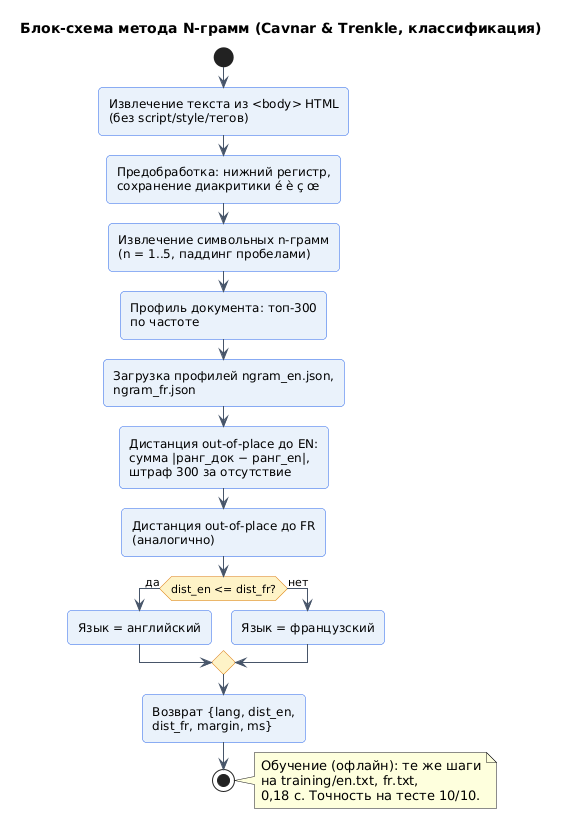
\includegraphics[width=0.62\textwidth]{png/activity_lang_ngram.png}
	\caption{Блок-схема метода N-грамм (классификация).}
	\label{fig:lang_ngram_flow}
\end{figure}

Обучение занимает 0,18~с (только стандартная библиотека Python).

\subsection{Алфавитный метод}

Французский язык обладает характерным признаком "--- буквами с диакритикой,
не встречающимися в исконно английских словах. Считаются: доля таких букв
среди всех букв текста и баланс слов-маркеров. Итоговый скор:

\begin{equation}
	S = 1{,}0 \cdot \frac{D}{N} + 0{,}5 \cdot \frac{F - E}{W},
	\label{eq:lang_alpha}
\end{equation}

где $D$ "--- число букв с диакритикой, $N$ "--- всех букв; $F$, $E$ "---
числа французских (\texttt{le/la/les/des/une/est/pour} и др.) и английских
(\texttt{the/and/of/to/in} и др.) маркеров; $W$ "--- всех слов.
Решение: французский при $S \ge T$, иначе английский. Порог $T = 0{,}04726$
подобран автоматически на обучающем корпусе как середина между худшим
скором FR-чанков и лучшим скором EN-чанков (классы разделились без
пересечений). Блок-схема "--- на рисунке~\ref{fig:lang_alpha_flow}.

\begin{figure}[H]
	\centering
	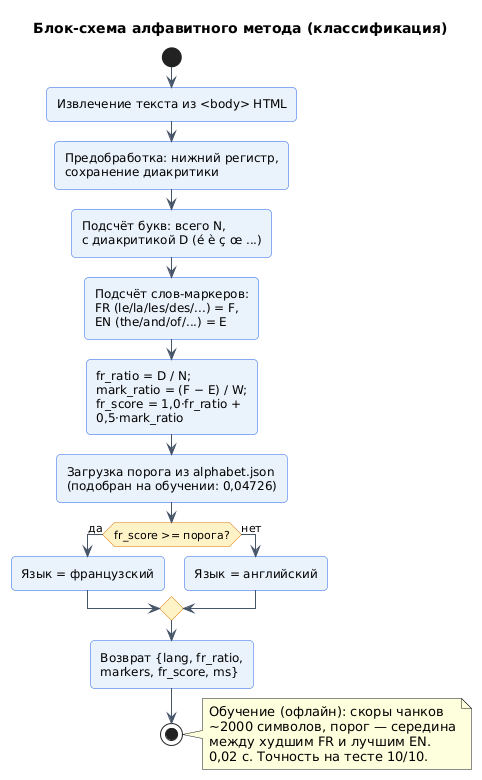
\includegraphics[width=0.62\textwidth]{png/activity_lang_alphabet.png}
	\caption{Блок-схема алфавитного метода (классификация).}
	\label{fig:lang_alpha_flow}
\end{figure}

Обучение (подбор порога) занимает 0,02~с.

\subsection{Нейросетевой метод}

Признаки "--- символьные TF-IDF (анализатор \texttt{char},
$n = 1\ldots5$, \texttt{max\_features}~=~5000); классификатор "---
логистическая регрессия (\texttt{max\_iter}~=~1000):

\begin{equation}
	P(\text{fr} \mid x) = \frac{1}{1 + \exp(-(w \cdot x + b))}.
	\label{eq:lang_logreg}
\end{equation}

Обучение "--- на чанках корпуса со стратифицированным holdout-контролем
80/20 (метрики \texttt{train\_accuracy} / \texttt{holdout\_accuracy}
сохраняются в метаданных модели). На выходе "--- вероятности $P(\text{EN})$
и $P(\text{FR})$. Метод требует scikit-learn (имеется в Docker-образе);
при отсутствии библиотеки остальные два метода продолжают работать,
голосование идёт по доступным.

\subsection{Эксперименты}

Тестовая коллекция (10 HTML-документов) прогнана скриптом
\texttt{backend/train\_lang\_model.py batch} (дублируется эндпоинтом
\texttt{/api/lang/classify-batch}). Результаты "--- в
таблице~\ref{tab:lang_results}.

\begin{table}[H]
	\caption{Точность и быстродействие методов (10 документов).}
	\label{tab:lang_results}
	\begin{tabular}{|l|l|l|}
		\hline
		Метод & Точность & Среднее время на документ \\ \hline
		N-граммы & 1,00 (10/10) & 7,89 мс \\
		Алфавитный & 1,00 (10/10) & 0,87 мс \\
		Нейросетевой & --- (прогон в Docker) & --- \\
		Голосование трёх (двух) методов & 1,00 (10/10) & 8,86 мс \\ \hline
	\end{tabular}
\end{table}

Confusion-матрицы обоих измеренных методов "--- идеальные:
$\begin{smallmatrix} 5 & 0 \\ 0 & 5 \end{smallmatrix}$
(строки "--- истина EN/FR, столбцы "--- предсказание EN/FR).
Методы сошлись на всех 10 документах (\texttt{agreed}~=~true).
Алфавитный метод на порядок быстрее N-граммного при равной точности
на данной коллекции; обучаются оба за доли секунды без сторонних
зависимостей. Строка нейросетевого метода заполняется после прогона
в Docker-контейнере (scikit-learn входит в образ); интерфейс отчёта
(CSV со столбцами предсказаний всех методов) уже выдаёт его колонку.

\subsection{Используемые библиотеки}

\begin{itemize}
	\item \textbf{scikit-learn} "--- \texttt{TfidfVectorizer} (символьные n-граммы) и \texttt{LogisticRegression} для нейросетевого метода; входит в \texttt{backend/requirements.txt}, в локальном интерпретаторе может отсутствовать "--- тогда доступны два остальных метода;
	\item стандартная библиотека Python (\texttt{re}, \texttt{html}, \texttt{json}, \texttt{collections}) "--- парсинг HTML, профили N-грамм, алфавитный скоринг: внешних зависимостей не требуют;
	\item \textbf{PlantUML} "--- исходники диаграмм \texttt{plantuml/sequence\_lang\_*.puml}, \texttt{plantuml/activity\_lang\_*.puml}, рендер в \texttt{png/} через публичный API.
\end{itemize}

\subsection{Выводы}

Переиспользовав клиент-серверную архитектуру ИПС, реализована подсистема
распознавания языка (вариант~7: французский/английский, HTML) тремя
методами с голосованием. Классификатор интегрирован в поисковый конвейер:
при загрузке документа язык классифицируется и записывается в колонку
\texttt{lang} таблицы \texttt{documents}; при поиске язык запроса
определяется автоматически; предобработка текста выбирается в зависимости
от языка. Измеренные на тестовой коллекции результаты: точность
N-граммного и алфавитного методов "--- 100\%, среднее время "--- единицы
миллисекунд; обучение "--- доли секунды. Подсистема устойчива к отсутствию
scikit-learn (деградация до двух методов), снабжена автообучением при старте,
CLI для офлайн-экспериментов, веб-интерфейсом с выгрузкой CSV-отчёта и
статической справкой.
